% LaTeX source for ``Algorithms for Computer Simulation of Molecular Systems''
% Copyright (c) 2023 รังสิมันต์ เกษแก้ว (Rangsiman Ketkaew).

% License: Creative Commons Attribution-NonCommercial-NoDerivatives 4.0 International (CC BY-NC-ND 4.0)
% https://creativecommons.org/licenses/by-nc-nd/4.0/

\chapter{การพัฒนาซอฟต์แวร์สำหรับเคมีเชิงคำนวณ}
\label{ch:software_dev}

%----------------------------------------
\section{การเขียนโปรแกรมทางเคมีเชิงคำนวณ}
%----------------------------------------

ถ้าหากผู้อ่านอยากจะศึกษาการเขียนโปรแกรมทางเคมีเชิงคำนวณจะเริ่มยังไงดี เช่น ต้องการเขียนโปรแกรม Density Functional Theory (DFT)
หรือ Implement วิธีโครงสร้างเชิงอิเล็กทรอนิกส์ (Electronic Structure) ผมขอให้ความเห็นอย่างนี้ครับว่าการจะที่เขียนโปรแกรมทางเคมี%
คำนวณขึ้นมาสักโปรแกรมหนึ่งนั้นใช้เวลามากพอสมควรเพราะว่ามีรายละเอียดที่ซับซ้อนมาก (เวลาที่ใช้ในการเขียนนั้นขึ้นอยู่กับว่าเขียนคนเดียวหรือช่วย%
กันเขียนหลายคน) ดังนั้นผมแนะนำว่าสำหรับผู้ที่เพิ่งเริ่มต้นการเขียนโปรแกรมทางวิทยาศาสตร์ควรศึกษาจากโปรแกรมมาตรฐานที่ได้รับความนิยมอยู่แล้ว
ผมไม่ได้บอกว่าห้ามเขียนโปรแกรมใหม่เองแบบเริ่มจากศูนย์หรือ From Scratch แต่ถ้าหากว่าเราเริ่มต้นเรียนรู้จากโปรแกรมที่ได้รับความนิยมและใช้งาน%
กันอย่างแพร่หลายอยู่แล้วก็มีข้อดีดังนี้

\begin{itemize}[topsep=0pt]
  \item ประหยัดเวลา ไม่ต้องมานั่งศึกษาหรือเขียนโค้ดใหม่เองทั้งหมด

  \item ได้เรียนรู้วิธีการเขียนโค้ดที่มีประสิทธิภาพจากนักพัฒนาคนอื่น ๆ

  \item เป็นการต่อยอดและพัฒนาโปรแกรมนั้น ๆ ให้ดีขึ้นไปอีกเพราะเราไม่จำเป็นต้องมา Reinvent the Wheel

  \item เป็นการสร้างเครือข่ายนักวิจัยและความร่วมมือทางวิชาการในระดับนานาชาติ
\end{itemize}

\noindent อย่างไรก็ตามถ้าหากใครอยากจะเริ่มเขียนโปรแกรมเองนั้น (ไม่จำเป็นต้องเป็น DFT อย่างเดียว แต่รวมถึงวิธีการจำลองทางคอมพิวเตอร์อื่น ๆ
ด้วย เช่น Molecular Dynamics หรือ Monte Carlo) ก็มีข้อดีหลายข้อเหมือนกัน ดังนี้

\begin{itemize}[topsep=0pt]
  \item ได้ทำความเข้าใจการเขียนโปรแกรมอ้างอิงตามสมการทาง Electronic Structure

  \item ฝึกทักษะการเขียนโปรแกรมสำหรับการคำนวณทางวิทยาศาสตร์และได้เรียนรู้เทคนิคการประมาณค่าเชิงตัวเลข

  \item ได้ออกแบบโปรแกรมเองและ Implement วิธีใหม่ ๆ ที่โปรแกรมอื่นไม่มี

  \item ต่อยอดเป็นโปรแกรมในรูปแบบเชิงพานิชย์ได้เพราะว่ามีโปรแกรมทางเคมีคำนวณหลาย ๆ โปรแกรมที่ขาย License
\end{itemize}

ประเด็นหรือคำถามสำคัญคือ \enquote{ถ้าหากอยากจะเริ่มศึกษาโค้ดของวิธีการคำนวณทางเคมีควอนตัม เช่น โปรแกรม Density Functional
  Theory (DFT) ดี ๆ สักตัวนึงจะเริ่มจากไหนดี?} ความเห็นของผมคือแนะนำให้ศึกษาโปรแกรม PySCF โดยมีเหตุผลดังต่อไปนี้

\begin{itemize}[topsep=0pt]
  \item โปรแกรมมีประสิทธิภาพสูง ทำงานได้เร็วและให้ผลการคำนวณที่ถูกต้องและแม่นยำและยังคำนวณได้หลากหลายวิธี

  \item มีผู้ใช้งานเยอะเนื่องจากว่าโปรแกรม PySCF นั้นสามารถติดตั้งและใช้งานได้ง่าย เตรียมไฟล์ Input ได้ไม่ยุ่งยาก

  \item PySCF เขียนด้วย Python เกือบทั้งหมด (87\% เขียนด้วย Python, 12\% เป็นภาษา C ก็คือพวกไลบรารี่ต่าง ๆ ที่เอามาคำนวณ%
        ในส่วนที่ Python อาจจะคำนวณได้ช้า) ดังนั้นจึงง่ายต่อการทำความเข้าใจ

  \item มีทีมพัฒนาที่ใหญ่และแข็งแกร่ง ได้รับการสนับสนุนฟีเจอร์และแก้ไข Bug อย่างต่อเนื่อง
\end{itemize}

\noindent จากข้อ 1 ถ้าหากเราต้องการ Implement วิธีหรือเทคนิคใหม่ ๆ เข้าไปใน PySCF ก็ทำได้ง่ายเพราะว่าเขียนด้วยภาษา Python
นอกจากนี้โปรแกรมยังสามารถทำงานด้วย GPU ได้ด้วย (มี Plugin พิเศษชื่อว่า gpu2pyscf) ตัวโค้ดถูกเขียนและได้รับการปรับปรุงมาเป็นอย่างดี
(Well-written) มีการวางโครงสร้างของโปรแกรมที่เรียบร้อย แบ่ง Methods ต่าง ๆ ออกเป็น Module ที่ชัดเจนและมีการจัดวาง Function
ที่เหมาะสม สำหรับผู้อ่านที่สนใจโปรแกรม PySCF ก็ไปดูได้ที่ \url{https://github.com/pyscf/pyscf}

เมื่อเราเลือกโปรแกรมได้แล้ว ขั้นตอนต่อมาก็คือพยายามทำความเข้าใจทฤษฎีของหัวข้องานวิจัยที่เราต้องการศึกษา พยายามหาว่าเราสามารถพัฒนา%
วิธีนั้น ๆ ได้อย่างไรเพื่อที่จะปรับปรุงให้มีความถูกต้องในการคำนวณมากขึ้นหรือหากรณีที่ทฤษฎีนั้นยังไม่ครอบคลุม ขั้นตอนต่อไปคือหาวิธีการแก้ไข%
ปัญหาหรือ Solution สำหรับการปรับปรุงทฤษฎีนั้นแล้วเขียนออกมาเป็นสมการทางคณิตศาสตร์ที่เราจะนำไป Implement ได้ ขั้นตอนต่อไปก็คือ%
การวางแผนการเขียนโปรแกรมซึ่งสามารถทำได้ด้วยการเขียนโค้ดเทียมหรือ Pseudo Code ก่อนที่เราจะ Implement จริง ๆ โดยเราจะต้องคิดเกี่ยว%
กับการวางโครงสร้างหรือ Structure ของโปรแกรม เช่น แบ่งโปรแกรมออกเป็นโปรแกรมย่อย ๆ หลายส่วน เช่น แบ่งเป็น modules, functions,
classes, หรือ types โดยเราควรจะต้องคำนึงถึงการพัฒนาโปรแกรมต่อไปในอนาคตด้วยว่าโปรแกรมของเรานั้นสามารถที่จะรองรับฟีเจอร์ใหม่ ๆ
ที่นักพัฒนาคนอื่น ๆ จะเข้ามาช่วยพัฒนาเพิ่มเติมได้

หลังจากที่เรา Implement เข้าไปในโปรแกรมเสร็จเรียบร้อยแล้วเราควรจะต้องมีการตรวจสอบการทำงานของโปรแกรมหรือฟังก์ชันต่าง ๆ อย่างสม่ำเสมอ%
เพื่อตรวจสอบค่าที่ได้จากคำนวณว่ามีความถูกต้องและมีความสมเหตุสมผลมากน้อยแค่ไหน เมื่อได้ค่าการคำนวณที่ถูกต้องแล้วขั้นตอนสุดท้ายก็คือการ%
ปรับปรุงหรือทำความสะอาดโค้ดให้มีประสิทธิภาพและอ่านได้ง่ายขึ้น ในขั้นตอนนี้เราสามารถเรียนรู้ได้จากการศึกษาโค้ดที่นักพัฒนาคนอื่นเขียนไว้ก็ได้%
ว่าเขาเขียนอย่างไร ใช้วิธีหรือเทคนิคอะไรที่ทำให้โค้ดรันได้เร็วและมีประสิทธิภาพ นอกจากนี้ยังมีสิ่งอื่น ๆ ที่เราควรจะต้องทำด้วย เช่น เขียน Comment
หรือทำเอกสารประกอบการใช้งาน (Documentation) เพื่อที่ว่าตัวเราเองหรือนักพัฒนาคนอื่น ๆ ที่มาอ่านหรือแก้ไขโค้ดของเรานั้นสามารถทำความ%
เข้าใจโค้ดได้ง่ายและไม่ต้องมานั่งศึกษาเองจากศูนย์

%----------------------------------------
\section{การวางโครงสร้างโปรแกรม}
%----------------------------------------

การที่เราจะเขียนโปรแกรมคำนวณทางวิทยาศาสตร์นั้นควรที่จะต้องมีการวางแผนให้ดีเพราะว่าเมื่อเราเขียนโค้ดไปเรื่อย ๆ ตัวโปรแกรมของเราก็จะมี%
ขนาดที่ใหญ่ขึ้นและมีความซับซ้อนมากขึ้นด้วย ดังนั้นการวางโครงสร้างของโปรแกรมเพื่อให้รองรับฟังก์ชันหรือฟีเจอร์ใหม่ ๆ ที่อาจจะมีการเขียนโค้ดเพิ่ม%
เข้ามานั้นช่วยให้โปรแกรมนั้นมีความเป็นระเบียบและง่ายต่อการ Maintenance และไม่สร้างความปวดหัวให้กับนักพัฒนาคนอื่น ๆ ที่อาจจะเข้ามาพัฒนา%
โปรแกรมของเราต่อ (อาจจะสร้างความปวดหัวแต่ก็ไม่เยอะเท่ากับโปรแกรมที่มีการวางโครงสร้างที่ไม่ดี)

ผมขอยกตัวอย่างโปรแกรม CP2K ซึ่งเป็นโปรแกรมที่ผมใช้ในงานทำวิจัย ตัว Source Code ของ CP2K นั้นจะมีโฟลเดอร์ต่าง ๆ เช่น src/, docs/,
tests/, หรือ tools/ ซึ่งโฟลเดอร์เหล่านี้เก็บไฟล์ที่มีหน้าที่แตกต่างกันออกไป แต่โฟลเดอร์ที่น่าจะสำคัญที่สุดก็คือ src/ ซึ่งเก็บไฟล์โค้ดการทำงานหลัก%
ของตัวโปรแกรมเอาไว้ ส่วนโฟลเดอร์อื่น ๆ เช่น test เป็นโฟลเดอร์ที่เก็บไฟล์อินพุตและเอาต์พุตที่ไว้ใช้สำหรับการทดสอบโปรแกรมและเปรียบเทียบกับ%
ค่าผลลัพธ์จากการคำนวณว่าได้ค่าที่ถูกต้องและแม่นยำ ตัวโฟลเดอร์ src/ นั้นบางโปรแกรมก็มีขนาดหลายร้อยเมกะไบต์หรือบางโปรแกรมก็มีหลายกิกะไบต์
ขึ้นอยู่กับว่าตัวโปรแกรมนั้นซับซ้อนมากแค่ไหน ซึ่งความซับซ้อนของโปรแกรมนั้นอาจจะวัดได้ง่าย ๆ จากจำนวนของฟีเจอร์หรือวิธีการที่โปรแกรมสามารถ%
คำนวณได้ นอกจากนี้เรายังดูได้จากความซับซ้อนของการ Implementation เช่น ถ้าโปรแกรมสามารถทำงานแบบขนาด (Parallel) บน Distributed
Cluster ได้นั่นหมายความว่าโค้ดของโปรแกรมนั้นจะต้องมีการถูกปรับ (Optimized) ให้รองรับวิธี OpenMP หรือ Message-passing Interface
(MPI) ซึ่งก็จะซับซ้อนกว่าโค้ดของโปรแกรมทั่วไป นอกจากนี้แล้วยังมีอีกหนึ่งเหตุผลนั่นก็คือโปรแกรมนั้นใช้ Packages หรือ Library อื่นมากน้อยแค่ไหน
เพราะว่าในปัจจุบันนั้นการพัฒนาโปรแกรมทางวิทยาศาสตร์โดยเฉพาะเคมีควอนตัมนั้นเราก็มักจะไม่ได้เขียนส่วนประกอบต่าง ๆ ของโปรแกรมเองใหม่ทั้งหมด
(หรือที่เรียกว่าเขียนแบบเริ่มจากศูนย์หรือ From Scratch เลย) นั่นก็เพราะว่าแต่ละส่วนหรือองค์ประกอบของการคำนวณนั้นมีความซับซ้อนมาก ดังนั้น%
จึงมีนักวิจัยที่สร้าง Library สำหรับการคำนวณบางอย่างไว้ให้เราแล้วซึ่งเราก็สามารถหยิบมาใช้ได้เลย การคำนวณบางอย่างที่มีความซับซ้อนนั้น เช่น
การคำนวณ Matrix Multiplication หรือการคำนวณ One-electron Integral และ Two-electron Integral รวมไปถึง Library
เฉพาะทาง เช่น Library ที่มีชุดฟังก์ชันของ DFT Functional ให้เรานำมาใช้งานได้เลย เรียกได้ว่าทำให้ชีวิตนักเคมีทฤษฎีที่ต้องพัฒนาโปรแกรมนั้น%
นั้นประหยัดเวลาชีวิตไปได้เยอะมาก โปรแกรม CP2K ซึ่งเป็นอีกหนึ่งโปรแกรมที่ถูกพัฒนาขึ้นโดยใช้ประโยชน์จาก Library อื่น ๆ มีโครงสร้างตามภาพ%
ด้านล่าง

\begin{figure}[htbp]
  \centering
  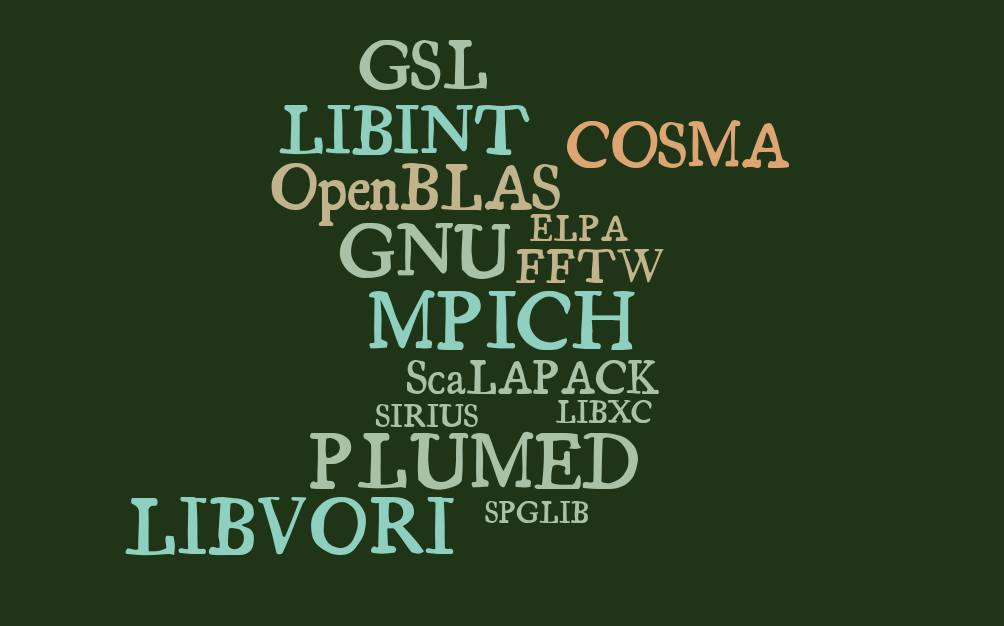
\includegraphics[width=0.7\linewidth]{fig/cp2k-lib.jpg}
  \caption{ไลบรารี่ที่โปรแกรม CP2K ใช้ในการช่วยคำนวณ}
  \label{fig:cp2k_lib}
\end{figure}

ผมจะมาอธิบายบาง Library ที่สำคัญ ๆ ของ CP2K ใช้ ดังนี้

\begin{description}
  \item[GNU] แน่นอนว่าเราต้องคอมไพล์ Source Code ดังนั้นเราจะต้องใช้ตัวคอมไพล์ (Compiler) ซึ่ง CP2K เลือกใช้ GNU เป็น Compiler

  \item[OpenBLAS กับ ScaLAPACK]  สำหรับ Linear Algebraic Calculation เช่น Matrix-vector, Matrix-matrix Multiplication

  \item[MPICH] อยากจะรันโปรแกรมแบบขนานโดยใช้ MPI ก็ต้องหา Implementation ที่จะมารันโค้ดของเรา ซึ่ง MPICH ก็เป็นหนึ่งใน
    Implementation ของ MPI ที่ CP2K เลือกใช้

  \item[FFTW] สำหรับทำฟูเรียร์ทรานฟอร์มในการคำนวณ DFT หรือแปลงจาก Real Space ไปเป็น Reciprocal Space สำหรับการคำนวณ
    Electrostatics โดยใช้ Plane Wave Electron Density

  \item[LIBXC] เป็น Library ที่ให้เราสามารถนำ DFT Functional มาใช้ได้เลยโดยไม่ต้อง Implement เอง
\end{description}

สรุปก็คือจะเห็นได้ว่าการเขียนโค้ดของโปรแกรมเคมีควอนตัมนั้นมีความซับซ้อนมากดังนั้นเรามีสองทางเลือกคือ

\begin{enumerate}[topsep=0pt,noitemsep]
  \setlength\itemsep{1em}
  \item ใช้ Library ที่มีอยู่แล้วสำหรับการทำงานเฉพาะจุด

  \item เขียนโค้ดทั้งหมดเองเลย
\end{enumerate}

แน่นอนว่าถ้าเราเลือกวิธีแรกก็จะประหยัดเวลาไปได้เยอะมากและเวลาที่เราคอมไพล์โปรแกรมก็ขอแค่ Link กับ Library ต่าง ๆ ก็รันโปรแกรมได้แล้ว%
และทำให้ขนาดของตัวโปรแกรมของเรา (ขนาดของ Binary Files) นั้นมีขนาดไม่ใหญ่มากเกินไปด้วย (เช่นหลักสิบ-ร้อยเมกะไบต์)

อย่างไรก็ตามโปรแกรมสำหรับจำลองระบบโมเลกุลหลาย ๆ โปรแกรมก็ไม่ได้ใช้ Library เหล่านี้และเลือกใช้วิธีที่ 2 ก็คือการเขียนโค้ดสำหรับการ%
คำนวณส่วนต่าง ๆ เองเลยเนื่องด้วยเหตุหลายข้อ เช่น การเขียนโค้ดทั้งหมดภายใน Framework โปรแกรมเดียวกันนั้นจะทำให้โค้ดมีประสิทธิภาพและ%
ทำงานร่วมกันได้ดี (Compatibility), ง่ายต่อการดูแลรักษาและปรับปรุงโค้ดเพราะว่า Developers นั้นรู้และเข้าใจการทำงานของโค้ดทั้งหมด,
ถึงแม้ว่าโปรแกรมที่เขียนโค้ดทั้งหมดเองเมื่อถูกคอมไพล์แล้วจะได้ออกมาเป็น Binary File ที่มีขนาดนั้นใหญ่มาก ๆ เช่น หลายกิกะไบต์ แต่ว่าก็มี%
ความคล่องตัวในการใช้งานเพราะว่าไม่ต้องติดตั้ง Library อื่น ๆ เพิ่มเติม

นอกจากนี้แล้วการที่ใช้ Library หลาย ๆ ตัวแบบนี้ก็มีจุดอ่อนบางข้อที่เราควรจะต้องรู้ไว้นั่นก็คือการเข้ากันได้ (Compatibility) ระหว่าง Library
หรือเวอร์ชันซึ่งก็อาจจะทำให้เราปวดหัวได้ถ้าหากว่า Library บางตัวมีการอัพเดทเวอร์ชันใหม่แล้ว Conflict กับ Library ตัวอื่น

%----------------------------------------
\section{ทักษะและเครื่องมือสำหรับการเขียนโปรแกรมคำนวณทางวิทยาศาสตร์}
%----------------------------------------

\noindent \textbf{ภาษาคอมพิวเตอร์}

\begin{itemize}[topsep=0pt]
  \item ภาษาสคริปต์ (Scripting Language): Bash, Python

  \item ภาษาระดับล่างที่เป็น Object-Oriented Programming: C++, Fortran

  \item ภาษาเชิงสัญลักษณ์ (Symbolic Programming): Mathematica, SymPy
\end{itemize}

\noindent \textbf{โปรแกรมสำหรับการเขียนโค้ด}

\begin{itemize}[topsep=0pt]
  \item Vi/Vim, Nano

  \item VS Code, Atom, Eclipse, Sublime, Notepad++
\end{itemize}

\noindent \textbf{พื้นฐานการเขียนโปรแกรม}

\begin{itemize}[topsep=0pt]
  \item ชนิดของตัวแปร (Variable Types)

  \item ตัวดำเนินการหรือโอเปอร์เรเตอร์ (Operator)

  \item Control Statements เช่น For, Do, If-Else, Case

  \item ฟังก์ชัน (Function)

  \item Vairable Scope และ Reference Types

  \item คลาส (Class) และวัตถุ (Objects)
\end{itemize}

\noindent \textbf{ภาษาคอมพิวเตอร์ระดับล่าง}

\noindent \underline{ภาษา C}

\begin{itemize}[topsep=0pt]
  \item Function, Pointer, Storage Class

  \item Enum, Struct, Union

  \item Preprocessor

  \item Operator, Memory Management, Array

  \item การจัดการไฟล์ (File Handling)
\end{itemize}

\noindent \textbf{ภาษาคอมพิวเตอร์ระดับสูง}

\noindent \underline{ภาษา Python}

\begin{itemize}[topsep=0pt]
  \item Pip และ Conda: ตัวช่วยจัดการไลบรารี่ของ Python

  \item NumPy: จัดการและคำนวณ Array (เวกเตอร์, เมทริกซ์)

  \item Numba: JIT Compiler สำหรับ NumPy

  \item Jax: ทำ Autograd (Gradient Comptuation) สำหรับ NumPy Array

  \item SciPy: ไลบรารี่ที่รวมรวบฟังก์ชันทางคณิตศาสตร์และวิทยาศาสตร์

  \item Scikit-learn: ไลบรารี่สำหรับทำสถิติ, Optimization, และ Curve Fitting รวมถึง Machine Learning

  \item Matplotlib, Plotly: พลอตกราฟ

  \item Theano: คำนวณเชิงตัวเลข (Numerical Computation)

  \item SCOOP: โมดูลสำหรับการทำโปรแกรมแบบขนาน (Parallel Programming)

  \item NetworkX: ไลบรารี่สำหรับ Graph
\end{itemize}

\noindent \underline{ภาษา C++}

\begin{itemize}[topsep=0pt]
  \item Type of variable: signed, unsigned, long, double, etc.

  \item Loops, conditional Statement

  \item Standard libraries: vector, rand

  \item Understanding header (`.hpp`) and source file (\texttt{.cpp} or \texttt{.cc})

  \item Preprocessor (\texttt{\#if}, \texttt{\#ifdef}, \texttt{\#ifndef}, \texttt{\#define}, etc.)

  \item Function, class, struct, template

  \item Declaration

  \item namespace, const, attribute, pointer, pass by reference, static_assert

  \item Initialization

  \item casting, lambda expression, encapsulation, file handling, exception handling
\end{itemize}

\noindent \underline{ภาษา Fortran}

\begin{itemize}[topsep=0pt]
  \item เรียนรู้ภาษา Fortran ที่เป็น Modern Fortran ตั้งแต่เวอร์ชัน 2003 เป็นต้นไป

  \item โมดูล (Module), โปรแกรมย่อยหรือซับรูทีน (Subroutine), ฟังก์ชัน (Function)

  \item Array ทั้งแบบที่ปรับเปลี่ยนได้ (Allocatable) และแบบหลายมิติ (Multidimentional)

  \item Operator Overloading, Flow control

  \item Derived Type

  \item Callback

  \item การเขียนโปรแกรมเชื่อมโยงกับภาษาอื่น เช่น Python หรือ C++

  \item การใช้ GNU Library ในการคอมไพล์

  \item การจัดการหน่วยความจำ (Memory Allocation): Stack, Heap, Global Memory
\end{itemize}

- Math Libraries
- BLAS (OpenBLAS)
- LAPACK for linear algebra
- ScaLAPACK - a higher level LAPACK
- Intel MKL (Intel oneAPI)
- FFTW: for computing the discrete Fourier transform in one or more dimensions, real and complex data
- Eigen: linear algebra library
- Boost: a collection of C++ functions e.g. `regex`, `serialization`

- QM Libraries
- libxc: XC function library
- libint: For computing Gaussian integral
- libcint: general GTO integrals

- Code Optimization
- Benchmarking และ Scaling
- Complexity (Big O)

- GNU
- Static and dynamic libraries
- Archive
- Compiling (g++, gcc) and linking (ld)
- Useful flags for compiler and linker e.g. `-O2`, `-O3`, `-fPIC`

- Compilng Tools
- autoconf
- configure
- Make, cmake, automake

- Debugging
- gdb for general debugging
- Valgrind for memory leak analysis

- Git (source code control)
- Basic/intermediate commands
- GitHub และ GitLab

- Documentation
- Sphinx (for markdown and reStructuredText)
- Doxygen

%----------------------------------------
\section{เขียนโปรแกรมวิเคราะห์ Molecular Geometry (ภาษา C++)}
%----------------------------------------

โปรแกรมอันแรกที่ผู้อ่านจะได้ฝึกเขียนตามก็คือโปรแกรมสำหรับวิเคราะห์เรขาคณิตเชิงโครงสร้าง Structural Geometry ของโมเลกุลโดยเราจะใช้%
ภาษา C++ กัน เหตุผลที่ผมเลือกใช้ภาษา C++ สำหรับการเขียนโปรแกรมแรกนี้ก็คืออยากให้ผู้อ่านได้ฝึกใช้ภาษา C++ ซึ่งเป็นภาษาที่มีประสิทธิภาพสูงมาก%
และถูกใช้อย่างแพร่หลายในการทำงานวิจัยเคมีควอนตัม (รวมถึงสาขาอื่น ๆ ด้วย) และโปรแกรมสำหรับการวิเคราะห์อันนี้ไม่มีความซับซ้อนมาก

\noindent \bful{Step 1: อ่านไฟล์ Coordinates}

\vspace{5pt}

\begin{lstlisting}[style=MyC++]
#include <iostream>
#include <fstream>
#include <iomanip>
#include <cstdio>

using namespace std;

int main() 
{
  ifstream input("geom.dat");

  int natom;
  input >> natom;

  int *zval = new int[natom];
  double *x = new double[natom];
  double *y = new double[natom];
  double *z = new double[natom];

  for(int i=0; i < natom; i++)
    input >> zval[i] >> x[i] >> y[i] >> z[i];
  
  input.close();

  cout << "Number of atoms: " << natom << endl;
  cout << "Input Cartesian coordinates:\n";
  for(int i=0; i < natom; i++)
    printf("%d %20.12f %20.12f %20.12f\n", (int) zval[i], x[i], y[i], z[i]);

  delete[] zval;
  delete[] x;  delete[] y;  delete[] z;

  return 0;
}
\end{lstlisting}

\vspace{5pt}

จากตัวอย่างโค้ดด้านบนนั้นเริ่มการทำงานด้วยการอ่านไฟล์ Coordinates ของอะตอมในโมเลกุลซึ่งมีหน่วยคือ bohr โดยผู้อ่านอาจจะลองใช้ตัวอย่าง%
โมเลกุลเล็ก ๆ เช่น Acetaldehyde ซึ่งมี Coordinates ดังนี้

\begin{Verbatim}[frame=single]
  7
  6  0.000000000000     0.000000000000     0.000000000000
  6  0.000000000000     0.000000000000     2.845112131228
  8  1.899115961744     0.000000000000     4.139062527233
  1 -1.894048308506     0.000000000000     3.747688672216
  1  1.942500819960     0.000000000000    -0.701145981971
  1 -1.007295466862    -1.669971842687    -0.705916966833
  1 -1.007295466862     1.669971842687    -0.705916966833
\end{Verbatim}

\noindent โดยที่เลข 7 ในบรรทัดแรกนั้นคือจำนวนอะตอมและบรรทัดที่เหลือนั้นคือพิกัดตำแหน่ง x, y, z ของอะตอมแต่ละตัว เมื่อโปรแกรมเปิดไฟล์%
แล้วสิ่งที่จะทำถัดไปก็คือการอ่านข้อมูลแต่ละบรรทัดและเก็บข้อมูลไว้ จริง ๆ แล้วเราสามารถ Simplify โค้ดตัวอย่างอันนี้ให้มีความเป็นระเบียบมากขึ้น%
โดยการใช้ Class เช่น เราสามารถสร้างไฟล์ header ที่ชื่อ \inlinehighlight{molecule.h} แล้วทำการเรียกใช้งาน Class ในไฟล์โปรแกรม
\inlinehighlight{molecule.cpp} ได้ดังนี้

\vspace{5pt}

\begin{lstlisting}[style=MyC++]
#include "molecule.h"
#include <iostream>
#include <fstream>
#include <iomanip>
#include <cstdio>

using namespace std;

int main()
{
  Molecule mol("geom.dat", 0);

  cout << "Number of atoms: " << mol.natom << endl;
  cout << "Input Cartesian coordinates:\n";
  mol.print_geom();

  return 0;
}
\end{lstlisting}

\vspace{5pt}

\noindent ทีนี้สิ่งที่ผมอยากให้ผู้อ่านทำก็คือลองฝึกเขียนโค้ดของไฟล์ \inlinehighlight{molecule.h} โดยดัดแปลงจากโค้ดด้านบนครับ

\noindent \bful{Step 2: คำนวณความยาวพันธะ (Bond Lengths)}

คำนวณระยะห่างระหว่างอะตอม (Interatomic Distances) โดยใช้สมการดังต่อไปนี้

\begin{equation}
  R_{ij}
  =
  \sqrt{
    (x_{i} - x_{j})^{2}
    + (y_{i} - y_{j})^{2}
    + (z_{i} - z_{j})^{2}
  }
\end{equation}

\noindent โดยที่ $x, y, z$ คือ Cartesian Coordinates และ $i$ กับ $j$ คือเลข Index ของอะตอม

สำหรับการเขียนโปรแกรมเพื่อคำนวณ Distance นั้นเราจะต้องคำนึงถึงการจัดการหน่วยความจำ (Memory Allocation) ด้วยเพื่อให้โปรแกรมของเรา%
นั้นมีประสิทธิภาพมากที่สุดซึ่งนั่นก็จะเกี่ยวข้องกับการเลือกวิธีในการเก็บข้อมูลของระยะห่างระหว่างอะตอม ในการหาความยาวระหว่างอะตอมของทุก ๆ
คู่นั้นสามารถใช้เมทริกซ์มาเก็บข้อมูลได้ซึ่งขนาดของเมทริกซ์จะเป็น $N \times N$ โดยที่ $N$ คือจำนวนอะตอม ในการใช้เมทริกซ์นั้นเราจำเป็นที่%
จะต้องจัดสรร (Allocate) หน่วยความจำซึ่งทำได้สองวิธีคือ

\noindent $\bullet$ 1. ใช้ Static Two-Dimensional Array

\vspace{5pt}

\begin{lstlisting}[style=MyC++]
double R[50][50];
\end{lstlisting}

\vspace{5pt}

\noindent $\bullet$ 2. ใช้ Dynamic Allocation โดยการใช้คลาส \inlinehighlight{Molecule}

\vspace{5pt}

\begin{lstlisting}[style=MyC++]
double **R = new double* [mol.natom];
for(int i=0; i < mol.natom; i++)
  R[i] = new double[mol.natom];
\end{lstlisting}

\vspace{5pt}

\noindent แล้วก็อย่าลืมลบหน่วยความจำหลังจากที่คำนวณเสร็จแล้วด้วย ดังนี้

\vspace{5pt}

\begin{lstlisting}[style=MyC++]
for(int i=0; i < mol.natom; i++)
  delete[] R[i];
delete[] R;
\end{lstlisting}

\vspace{5pt}

ขั้นตอนต่อไปก็คือการสร้างเมทริกซ์ขึ้นมาซึ่งสามารถทำได้โดยใช้ For Loop ในการวนไปเรื่อย ๆ ตามเลข Index ของอะตอม

\vspace{5pt}

\noindent แล้วก็อย่าลืมลบหน่วยความจำหลังจากที่คำนวณเสร็จแล้วด้วย ดังนี้

\vspace{5pt}

\begin{lstlisting}[style=MyC++]
...
#include <cmath>
...

for(int i=0; i < mol.natom; i++) {
  for(int j=0; j < mol.natom; j++) {
      R[i][j] = 
        sqrt(
          (mol.geom[i][0]-mol.geom[j][0])*(mol.geom[i][0]-mol.geom[j][0])
        + (mol.geom[i][1]-mol.geom[j][1])*(mol.geom[i][1]-mol.geom[j][1])
        + (mol.geom[i][2]-mol.geom[j][2])*(mol.geom[i][2]-mol.geom[j][2]) 
        );
  }
}
\end{lstlisting}

\vspace{5pt}

ลำดับต่อไปคือการแสดงค่าความยาวที่คำนวณได้โดยเราก็จะใช้ For Loop เหมือนเดิม

\vspace{5pt}

\begin{lstlisting}[style=MyC++]
for(int i=0; i < mol.natom; i++)
  for(int j=0; j < i; j++)
    printf("%d %d %8.5f\n", i, j, R[i][j]);
\end{lstlisting}

\vspace{5pt}

ขั้นตอนสุดท้ายคือการทำให้โค้ดนั้นมีความเรียบร้อยและมีประสิทธิภาพมากขึ้น โดยเราสามารถนำโค้ดด้านบนที่เราได้เขียนไว้สร้างเป็นฟังก์ชันใหม่ที่ชื่อว่า
\ih{bond()} ในคลาส \ih{Molecule} ได้ดังนี้

\vspace{5pt}

\begin{lstlisting}[style=MyC++]
double Molecule::bond(int a, int b)
{
  return sqrt( (geom[a][0]-geom[b][0])*(geom[a][0]-geom[b][0])
              + (geom[a][1]-geom[b][1])*(geom[a][1]-geom[b][1])
              + (geom[a][2]-geom[b][2])*(geom[a][2]-geom[b][2]) );
}
\end{lstlisting}

\vspace{5pt}

แล้วก็โปรแกรมของเราก็จะมีหน้าตาเป็นแบบนี้

\vspace{5pt}

\begin{lstlisting}[style=MyC++]
#include "molecule.h"
#include <iostream>
#include <fstream>
#include <iomanip>
#include <cstdio>
#include <cmath>

using namespace std;
  
int main()
{
  Molecule mol("geom.dat", 0);
  
  cout << "Number of atoms: " << mol.natom << endl;
  cout << "Input Cartesian coordinates:\n";
  mol.print_geom();
  
  cout << "\nInteratomic distances (bohr):\n";
  for(int i=0; i < mol.natom; i++)
    for(int j=0; j < i; j++)
      printf("%d %d %8.5f\n", i, j, mol.bond(i,j));
      
  return 0;
}
\end{lstlisting}

\vspace{5pt}

\noindent ซึ่งก็จะมีเอาต์พุตดังต่อไปนี้

\vspace{5pt}

\begin{lstlisting}[style=MyC++]
Number of atoms: 7
Input Cartesian coordinates:
6     0.000000000000     0.000000000000     0.000000000000
6     0.000000000000     0.000000000000     2.845112131228
8     1.899115961744     0.000000000000     4.139062527233
1    -1.894048308506     0.000000000000     3.747688672216
1     1.942500819960     0.000000000000    -0.701145981971
1    -1.007295466862    -1.669971842687    -0.705916966833
1    -1.007295466862     1.669971842687    -0.705916966833

Interatomic distances (bohr):
1 0  2.84511
2 0  4.55395
2 1  2.29803
3 0  4.19912
3 1  2.09811
3 2  3.81330
4 0  2.06517
4 1  4.04342
4 2  4.84040
4 3  5.87463
5 0  2.07407
5 1  4.05133
5 2  5.89151
5 3  4.83836
5 4  3.38971
6 0  2.07407
6 1  4.05133
6 2  5.89151
6 3  4.83836
6 4  3.38971
6 5  3.33994
\end{lstlisting}

\vspace{5pt}

\noindent โดยที่ \ih{bond()} คือ Member Function ของ \ih{Molecule} ซึ่งเราสามารถเรียกใช้ข้อมูลของ Geometry (Coordinates)
ได้ผ่าน \ih{geom} โดยไม่จำเป็นต้องเรียกใช้ผ่าน \ih{mol.geom}

\noindent \bful{Step 3: คำนวณมุมพันธะ (Bond Angles)}

เราสามารถคำนวณมุมพันธะทุกมุมที่เป็นไปได้ทั้งหมดของโมเลกุล (ระหว่างอะตอม $i, j, k$) $\phi_{ijk}$ ได้ด้วยสมการดังต่อไปนี้

\begin{equation}
  \label{eq:cos_bond_angle}
  \cos \phi_{ijk} = \tilde{e}_{ji} \cdot \tilde{e}_{jk}
\end{equation}

\noindent โดยที่ $e_{ij}$ คือเวกเตอร์หนึ่งหน่วย (Unit Vector) ระหว่างอะตอมซึ่งสามารถคำนวณได้ด้วยสมการดังต่อไปนี้

\begin{align*}
  e^{x}_{ij}
  = \frac{
    -(x_{i} - x_{j})
  }
  {
    R_{ij}
  } \\
  e^{y}_{ij}
  = \frac{
    -(y_{i} - y_{j})
  }
  {
    R_{ij}
  } \\
  e^{z}_{ij}
  = \frac{
    -(z_{i} - z_{j})
  }
  {
    R_{ij}
  }
\end{align*}

\vspace{5pt}

โดยเราจะสร้างฟังก์ชันสำหรับคำนวณมุมพันธะซึ่งก็คือ Inverse ของฟังก์ชัน Cosine ของสมการที่ \eqref{eq:cos_bond_angle} แล้วเพิ่มฟังก์ชัน%
นี้เข้าไปในไฟล์ \ih{molecule.cpp} ดังนี้

\vspace{5pt}

\begin{lstlisting}[style=MyC++]
// Returns the value of the unit vector between atoms a and b
// in the cart direction (cart=0=x, cart=1=y, cart=2=z)
double Molecule::unit(int cart, int a, int b)
{
  return -(geom[a][cart]-geom[b][cart])/bond(a,b);
}

// Returns the angle between atoms a, b, and c in radians
double Molecule::angle(int a, int b, int c)
{
  return acos(unit(0,b,a) * unit(0,b,c) + unit(1,b,a) * unit(1,b,c) + unit(2,b,a) * unit(2,b,c));
}
\end{lstlisting}

\vspace{5pt}

\noindent นอกจากนี้เราจะต้องเพิ่ม Declaration ของ Member Function เข้าไปในไฟล์ \ih{molecule.h} ด้วย ดังนี้

\vspace{5pt}

\begin{lstlisting}[style=MyC++]
#include <string>

using namespace std;

class Molecule
{
  public:
    int natom;
    int charge;
    int *zvals;
    double **geom;
    string point_group;

    void print_geom();
    void rotate(double phi);
    void translate(double x, double y, double z);
    double bond(int atom1, int atom2);
    double angle(int atom1, int atom2, int atom3);
    double torsion(int atom1, int atom2, int atom3, int atom4);
    double unit(int cart, int atom1, int atom2);

    Molecule(const char *filename, int q);
    ~Molecule();
};
\end{lstlisting}

\vspace{5pt}

แล้วโปรแกรมสำหรับคำนวณมุมพันธะที่สมบูรณ์นั้นจะมีหน้าตาแบบนี้

\vspace{5pt}

\begin{lstlisting}[style=MyC++]
#include "molecule.h"
#include <iostream>
#include <fstream>
#include <iomanip>
#include <cstdio>
#include <cmath>

using namespace std;
  
int main()
{
  Molecule mol("geom.dat", 0);
  
  cout << "Number of atoms: " << mol.natom << endl;
  cout << "Input Cartesian coordinates:\n";
  mol.print_geom();

  cout << "\nBond angles:\n";
  for(int i=0; i < mol.natom; i++) {
    for(int j=0; j < i; j++) {
      for(int k=0; k < j; k++) {
        if(mol.bond(i,j) < 4.0 && mol.bond(j,k) < 4.0)
          printf("%2d-%2d-%2d %10.6f\n", i, j, k, mol.angle(i,j,k)*(180.0/acos(-1.0)));
      }
    }
  }

  return 0;
}
\end{lstlisting}

\vspace{5pt}

\noindent โดยที่เราใช้ \cppinline{acos(-1.0)} ในการประมาณค่า $\pi$

เมื่อเรารันโปรแกรมด้านบนจะได้เอาต์พุตแบบนี้

\vspace{5pt}

\begin{lstlisting}
Number of atoms: 7
Input Cartesian coordinates:
6     0.000000000000     0.000000000000     0.000000000000
6     0.000000000000     0.000000000000     2.845112131228
8     1.899115961744     0.000000000000     4.139062527233
1    -1.894048308506     0.000000000000     3.747688672216
1     1.942500819960     0.000000000000    -0.701145981971
1    -1.007295466862    -1.669971842687    -0.705916966833
1    -1.007295466862     1.669971842687    -0.705916966833

Bond angles:
  2- 1- 0 124.268308
  3- 1- 0 115.479341
  3- 2- 1  28.377448
  5- 4- 0  35.109529
  6- 4- 0  35.109529
  6- 5- 0  36.373677
  6- 5- 4  60.484476
\end{lstlisting}

\vspace{5pt}

\noindent \bful{Step 4: คำนวณมุมบิด (Torsion หรือ Dihedral Angles)}

พารามิเตอร์ลำดับต่อมาที่เราจะคำนวณก็คือมุมบิด (Torsion Angle) สำหรับมุมบิดของอะตอม 4 อะตอมใด ๆ ในโมเลกุล $i, j, k, l$ นั้นมี%
สมการในการคำนวณคือ

\begin{equation}
  \cos \tau_{ijkl}
  =
  \frac{
    (\tilde{e}_{ij} \times \tilde{e}_{jk})
    \cdot
    (\tilde{e}_{jk} \times \tilde{e}_{kl})
  }
  {
    \sin \theta_{ijk}
    \sin \theta_{jkl}
  }
\end{equation}

\noindent สิ่งที่ต้องระวังในการคำนวณ Torsion Angle ก็คือเครื่องหมายของมุมซึ่งจะเป็นบวกหรือลบนั้นก็คือขึ้นอยู่กับว่าเวกเตอร์นั้นมีทิศทางไปทาง%
ไหนเมื่อเทียบกับระนาบ

\begin{itemize}[topsep=0pt,noitemsep]
  \setlength\itemsep{1em}
  \item มุมบิดของอะตอม $i-j-k-l$ เป็นบวกเมื่อเวกเตอร์ตามแนวอะตอม $k-l$ นั้นวางตัวไปทางด้านขวาของระนาบที่สร้างจากอะตอม $i-j-k$
        เมื่อมองจากทิศทางของเวกเตอร์ $j-k$

  \item มุมบิดของอะตอม $i-j-k-l$ เป็นลบเมื่อเวกเตอร์ตามแนวอะตอม $k-l$ นั้นวางตัวไปทางด้านซ้ายของระนาบที่สร้างจากอะตอม $i-j-k$
        เมื่อมองจากทิศทางของเวกเตอร์ $j-k$
\end{itemize}

\vspace{5pt}

โปรแกรมสำหรับคำนวณ Torsion Angle นั้นมีดังนี้ เริ่มต้นด้วยการสร้าง Member Function ของคลาส \ih{Molecule}

\vspace{5pt}

\begin{lstlisting}[style=MyC++]
// Computes the angle between planes a-b-c and b-c-d
double Molecule::torsion(int a, int b, int c, int d)
{
  double eabc_x = (unit(1,b,a)*unit(2,b,c) - unit(2,b,a)*unit(1,b,c));
  double eabc_y = (unit(2,b,a)*unit(0,b,c) - unit(0,b,a)*unit(2,b,c));
  double eabc_z = (unit(0,b,a)*unit(1,b,c) - unit(1,b,a)*unit(0,b,c));

  double ebcd_x = (unit(1,c,b)*unit(2,c,d) - unit(2,c,b)*unit(1,c,d));
  double ebcd_y = (unit(2,c,b)*unit(0,c,d) - unit(0,c,b)*unit(2,c,d));
  double ebcd_z = (unit(0,c,b)*unit(1,c,d) - unit(1,c,b)*unit(0,c,d));

  double exx = eabc_x * ebcd_x;
  double eyy = eabc_y * ebcd_y;
  double ezz = eabc_z * ebcd_z;

  double tau = (exx + eyy + ezz)/(sin(angle(a,b,c)) * sin(angle(b,c,d)));

  if(tau < -1.0) tau = acos(-1.0);
  else if(tau > 1.0) tau = acos(1.0);
  else tau = acos(tau);

  // Compute the sign of the torsion 
  double cross_x = eabc_y * ebcd_z - eabc_z * ebcd_y;
  double cross_y = eabc_z * ebcd_x - eabc_x * ebcd_z;
  double cross_z = eabc_x * ebcd_y - eabc_y * ebcd_x;
  double norm = cross_x*cross_x + cross_y*cross_y + cross_z*cross_z;
  cross_x /= norm;
  cross_y /= norm;
  cross_z /= norm;
  double sign = 1.0;
  double dot = cross_x*unit(0,b,c)+cross_y*unit(1,b,c)+cross_z*unit(2,b,c);
  if(dot < 0.0) sign = -1.0;

  return tau*sign;
}
\end{lstlisting}

\vspace{5pt}

แล้วเราก็เรียกใช้ฟังก์ชันใหม่ที่เราเพิ่งสร้างไว้ในโปรแกรมหลักของเราได้ดังนี้

\vspace{5pt}

\begin{lstlisting}[style=MyC++]
#include <iostream>
#include <fstream>
#include <iomanip>
#include <cstdio>
#include <cmath>
#include "molecule.h"

using namespace std;

int main()
{
  Molecule mol("geom.dat", 0);

  cout << "Number of atoms: " << mol.natom << endl;
  cout << "Input Cartesian coordinates:\n";
  mol.print_geom();

  cout << "\nTorsional angles:\n";
  for(int i=0; i < mol.natom; i++) {
    for(int j=0; j < i; j++) {
      for(int k=0; k < j; k++) {
        for(int l=0; l < k; l++) {
          if(mol.bond(i,j) < 4.0 && mol.bond(j,k) < 4.0 && mol.bond(k,l) < 4.0)
            printf("%2d-%2d-%2d-%2d %10.6f\n", i, j, k, l, mol.torsion(i,j,k,l)*(180.0/acos(-1.0)));
        }
      }
    }
  }

  return 0;
}
\end{lstlisting}

\vspace{5pt}

\noindent เมื่อเรารันโปรแกรมด้านบนเราจะได้เอาต์พุตดังนี้

\vspace{5pt}

\begin{lstlisting}[style=MyC++]
Number of atoms: 7
Input Cartesian coordinates:
6       0.000000000000       0.000000000000       0.000000000000
6       0.000000000000       0.000000000000       2.845112131228
8       1.899115961744       0.000000000000       4.139062527233
1      -1.894048308506       0.000000000000       3.747688672216
1       1.942500819960       0.000000000000      -0.701145981971
1      -1.007295466862      -1.669971842687      -0.705916966833
1      -1.007295466862       1.669971842687      -0.705916966833

Torsional angles:
  3- 2- 1- 0 180.000000
  6- 5- 4- 0  36.366799  
\end{lstlisting}

\vspace{5pt}

\noindent \bful{Step 5: คำนวณจุดศูนย์กลางมวล มุมบิด (Center of Mass)}

\noindent แบบฝึกหัด: ผมอยากผู้อ่านลองเขียนโปรแกรมคำนวณจุดศูนย์กลางมวลของโมเลกุล

\vspace{5pt}

%----------------------------------------
\section{เขียนโปรแกรม Hartree-Fock SCF (ภาษา Python)}
%----------------------------------------

โปรแกรมเคมีควอนตัมทุกโปรแกรมจะต้องมีส่วนหนึ่งของโปรแกรมที่เป็นโค้ดสำหรับแก้สมการอันหนึ่งซึ่งขาดไม่ได้เลยนั่นก็คือ Roothaan-Hall
Equation โดยใช้วิธี Self-Consistent Field ซึ่งเป็นสมการที่เราใช้ในการคำนวณหาพลังงานของระบบที่เราสนใจ

สมการ Roothaan-Hall นั้นจะเรียกว่าเป็นสมการ HF ที่แปลงร่างมาแล้วก็ได้ สาเหตุที่เราต้องทำการแปลงร่าง HF นั้นก็เพราะว่าเราเขียน
Wavefunction ให้อยู่ในรูปที่มี Basis Function นั่นเอง (Basis Function คือสิ่งที่เราใช้อธิบายออร์บิทัลเชิงอะตอม) โดยเราจะมีสมการ
Roothaan-Hall ทั้งหมด $m$ สมการ โดยที่ $m$ คือจำนวนของ Basis Function (เรามีสมการ HF 1 สมการต่อ 1 MO และการที่เรามี
$m$ Basis Function นั้นก็จะสร้างทั้งหมด $m$ MOs ด้วย), $F$ คือ Fock Matrix ซึ่งก็จะได้จาก Density Matrix แล้ว
Density Matrix ก็คือ Matrix ที่มีสมาชิกเป็นผลคูณระหว่าง Coefficients ของ MO ซึ่งก็จะได้มาจากการประมาณค่าด้วยวิธีเริ่มต้น
(Initial Guess) แบบต่าง ๆ เช่นใช้ Huckel Method, ส่วน $S$ นั้นก็คือ Overlap Matrix ซึ่งก็จะเป็น Matrix ที่บอกว่า
Orbitals นั้นสัมพันธ์กันมากน้อยแค่ไหน, และ $\epsilon$ ของแต่ละสมการนั้นก็คือค่าพลังงานของแต่ละ MO นั้นเองซึ่งเป็นสิ่งที่เรา%
ต้องการแก้สมการหามันออกมา

ทีนี้เราสามารถยุบรวมสมการทั้งหมดในรูปที่ 1 ได้ออกมาเป็นตามสมการที่สั้นและกระชับขึ้นตามรูปที่ 2 ซึ่ง $F$, $C$, และ $S$ นั้นเป็น Matrix
ที่มีขนาดคือ $m \times m$ แล้วก็ epsilon นั้นก็มีขนาด $m \times m$ ด้วย (จะมีเฉพาะสมาชิกในแนวทแยงเท่านั้นที่มีค่าไม่เท่ากับ 0)
โดยเราสามารถแสดงสมการด้านซ้ายและขวาให้เป็น Matrix ได้ตามรูปที่ 3 และ 4

ประเด็นอยู่ตรงนี้ก็คือตามวิชา Linear Algebra ถ้าเราต้องการหา Matrix ของ $\epsilon$ เราสามารถใช้วิธี Diagonalization
กับสมการ Roothaan-Hall ได้เพราะว่าสมการนี้มันเป็น Eigenfunction ซึ่งกระบวนกานที่จะใช้ในการแก้นั้นก็คือตามขั้นตอนต่อไปนี้

\noindent \textbf{กระบวนการ SCF:}

\begin{enumerate}[topsep=0pt,noitemsep]
  \setlength\itemsep{1em}
  \item เรากำหนดตำแหน่งของอะตอมในโมเลกุล, ประจุ, และทำการเลือก Basis Set

  \item เริ่มคำนวณพลังงานจลน์และพลังงานศักย์ รวมไปถึง Overlap Integral

  \item คำนวณ Orthogonalizing Matrix โดยใช้ Overlap Matrix (Overlap Matrix ที่ถูกสร้างมาจาก Overlap Integral
        ที่ได้จากขั้นที่ 2 อีกที)

  \item คำนวณ Fock Matrix อันแรกเลยโดยใช้พลังงานจลน์และพลังงานศักย์แล้วก็ใช้ Initial Guess ที่ได้จาก Coefficients
        ของ Basis Set ที่กำหนดไว้ตั้งแต่ขั้นตอนที่ 1

  \item ใช้ Orthogonalizing Matrix เพื่อแปลง (Tranform) Fock Matrix ให้เป็น Matrix อันใหม่ (เรียกว่าเป็น $F'$ ก็แล้วกัน)
        ที่มันขึ้นอยู่กับ Orthogonal Set ของฟังก์ชันที่ได้มาจาก Basis Set ที่ถูกเซนเตอร์กับอะตอม (Atom-centered Basis Set)

  \item ทำการทำเมทริกซ์แนวทแยง (Diagonalize) Fock Matrix เพื่อหา Coefficient Matrix ที่ถูกแปลงมาแล้ว (เรียกว่า $C'$)
        ก็ได้แล้วก็หาพลังงานของแต่ละ MO ได้

  \item เปรียบเทียบ $C'$ และพลังงานกับค่าที่ได้จากรอบก่อนหน้านี้ ถ้าผลต่างยังไม่น้อยกว่า Cutoff ที่กำหนดไว้ก็ให้นำ Fock Matrix
        ที่ได้มาล่าสุดไปใช้ใหม่อีกครั้งหนึ่งในขั้นที่ 4 ทำวนไปเรื่อย ๆ จนได้คำตอบที่แม่นยำ
\end{enumerate}

สำหรับการกำหนด Basis Set นั้นก็คือการเลือกชุดค่าสัมประสิทธิ์ของออร์บิทัล (Wavefunction) ของธาตุแต่ละธาตุ จริง ๆ แล้ว Basis Set
นั้นก็คือไฟล์ Text ที่มีรูปแบบ (Format) ที่แตกต่างกันไปตามโปรแกรมที่ใช้ เราสามารถดาวน์โหลดไฟล์ Basis Set ได้ที่เว็บไซต์
\url{https://www.basissetexchange.org/} ตัวอย่างเช่น Basis Set: aug-cc-PV7Z ของอะตอมคาร์บอน
\url{https://www.basissetexchange.org/basis/aug-cc-pv7z/format/nwchem/?version=0&elements=6}

%----------------------------------------
\section{เขียนโปรแกรมคำนวณ M\o{}ller-Plesset Perturbation (ภาษา Python)}
%----------------------------------------

%----------------------------------------
\section{เขียนโปรแกรมคำนวณ Coupled Cluster (ภาษา Python)}
%----------------------------------------

Coupled Cluster with Singles and Doubles (CCSD)

%----------------------------------------
\section{เขียนโปรแกรมคำนวณ DFT (ภาษา Python)}
%----------------------------------------

%----------------------------------------
\subsection{เขียนโปรแกรมคำนวณ Kohn-Sham Matrix}
%----------------------------------------

%----------------------------------------
\subsection{เขียนโปรแกรมฟังก์ชันนอล LDA}
%----------------------------------------

%----------------------------------------
\subsection{เขียนโปรแกรมฟังก์ชันนอล B3LYP}
%----------------------------------------

%----------------------------------------
\section{เขียนโปรแกรมคำนวณ Molecular Quantum Integrals }
%----------------------------------------

ในหัวข้อนี้ผู้อ่านจะได้เรียนรู้การเขียนโปรแกรมเพื่อคำนวณเทอม Molecular Integrals แบบต่าง ๆ ที่ใช้ Gaussian Basis Functions

%----------------------------------------
\subsection{ความรู้ทางคณิตศาสตร์ที่ต้องใช้}
%----------------------------------------

%----------------------------------------
\subsection{Overlap Integrals}
%----------------------------------------

%----------------------------------------
\subsection{Kinetic Energy Integrals}
%----------------------------------------

%----------------------------------------
\subsection{Nuclear Attraction Integrals}
%----------------------------------------

%----------------------------------------
\subsection{Two-Electron Repulsion Integrals}
%----------------------------------------

%----------------------------------------
\section{เขียนโปรแกรม DIIS สำหรับกระบวนการ SCF (ภาษา C++)}
%----------------------------------------

%----------------------------------------
\section{คำแนะนำสำหรับการคำนวณเคมีควอนตัม}
%----------------------------------------

คนที่ทำวิจัยด้านเคมีควอนตัมก็จะมีเทคนิคหรือแนวทางในการทำการคำนวณเคมีควอนตัมของตนเอง ขึ้นอยู่กับหลายปัจจัย ตัวอย่างเช่น เรียนจากคอร์ส%
ของมหาวิทยาลัย, อ่านจากหนังสือหรือตำราต่างประเทศที่ต่างกัน, ได้รับคำชี้แนะจากการทำวิจัยจากหลาย ๆ คน รวมถึงประสบการณ์หรือความเคยชิน%
กับโปรแกรมเคมีควอนตัมที่ตนเองถนัด อย่างไรก็ตาม ผมคิดว่าเราทุกคนควรจะต้องมีหลักการทางทฤษฎีที่ถูกต้องที่ควรจะต้องปฏิบัติตามกัน ซึ่งก็คือการเข้า%
ใจทฤษฎีทางเคมีควอนตัมและโครงสร้างเชิงอิเล็กทรอนิกส์ ในหัวนี้ผู้อ่านได้จะศึกษาแนวทางสำหรับการคำนวณเคมีควอนตัม

\paragraph{1. การเตรียม Input File โครงสร้างของโมเลกุลและการเลือก Electronic State}
ผมขอเริ่มด้วยสิ่งที่เป็นพื้นฐานที่สุดนั่นก็คือการเตรียมไฟล์อินพุต (Input) ซึ่งปรกติแล้วเรามักจะทราบกันดีว่าเราสามารถแสดง (Represent)
โครงสร้างของโมเลกุลได้ด้วยรูปแบบ (Format) 2 อัน นั่นคือ Cartesian (xyz) Format กับ z-matrix Format โดยใน xyz Format
นั้นเราจะใส่ลิสต์รายละเอียดของอะตอมในโมเลกุลนั่นคือเลขอะตอมและพิกัด Cartesian Coordinate ของอะตอมแต่ละตัว ส่วนใน z-matrix
Format นั้นจะเป็นการกำหนดโครงสร้างหรือ Geometry โดยการใช้พิกัดภายใน (Internal Coordinates) เช่น ควาามยาวพันธะ มุมพันธะ
และมุมบิด โดยโปรแกรมควอนตัมเคมีส่วนใหญ่นั้นทำการกำหนดรูปแบบเริ่มต้นของโครงสร้างโมเลกุลเป็นแบบพิกัด xyz รวมถึงพารามิเตอร์อื่น ๆ
เช่น กำหนดหน่วยเป็น Angstroms แต่ว่าโปรแกรมแต่ละโปรแกรมนั้นก็มักจะมีคีเวิร์ดให้สลับไปใช้หน่วยอื่น เช่น bohr พารามิเตอร์ที่สำคัญอีก 2
อันก็คือ Charge กับ Spin Multiplicity ของ Electronic State ที่เราสนใจที่จะศึกษา โดยประจุนั้นเป็นการระบุถึงจำนวนของอิเล็กตรอน
ส่วน Spin Multiplicity หาได้จากจำนวนรูปแบบที่อิเล็กตรอนสามารถจัดคู่ได้ซึ่งเขียนแทนด้วย $\ket{\Psi}$ สำหรับแต่ละ Configuration
นั่นเอง ตัวอย่างเช่น โมเลกุลมีเทน \ce{CH4} เรากำหนดประจุเป็น 0 ส่วน Spin Multiplicity นั้นเป็น 1 เพราะว่าจำนวน Alpha Electron
กับ Beta Electron นั้นเท่ากันใน Singlet State ดังนั้นจึงมี Configuration ได้แบบเดียว

\paragraph{2. การเลือก Basis Set}
ลำดับต่อมาคือเราจะต้องเลือก Basis Set ที่ต้องการใช้ อันนี้ก็เป็นปัญหาโลกแตกอีกอันหนึ่งในทางเคมีควอนตัม แต่ละคนก็จะมี Basis Set
ที่ตัวเองชอบหรือจะต้องใช้ Basis Set ที่โดนบังคับให้ใช้ อย่างไรก็ตาม ผมขำแบ่งคำแนะนำเบื้องต้นในการเลือก Basis Set ออกเป็น 2 กลุ่มหลัก ๆ
คือ Basis Set สำหรับการคำนวณด้วย DFT Method และด้วย Wavefunction-based Method

\begin{enumerate}
  \item สำหรับการคำนวณ Density Functional Theory (DFT) และ Hartree-Fock (HF) นั้นเรามักจะมีตัวเลือกทั่ว ๆ ไป เช่น
        6-31G(d), 6-31G(d,p) แต่ถ้าเป็นไปได้ก็ไปใช้ Basis Set อื่นที่ใหม่กว่านี้ดีกว่า (มีบทความวิชาการรีวิวที่ให้เหตุผลว่าทำไมเราถึงไม่ควรใช้
        Pople's Basis ตัวเล็ก ๆ) ถ้าเป็นไปได้ให้ลองใช้ Basis Set จากสำนัก Karlsruhe เช่น def2-SVP, def2-TZVP, def2-QZVP
        ถ้าหากว่าเราต้องมีการคำนวณเยอะมาก ๆ ผมแนะนำตัว def2-TZVP เพราะว่าจะให้ผลการคำนวณทั้งหมดที่ Converge ดีกว่า

  \item สำหรับ Wavefunction-based Method เช่น MP2, CCSD, CCSD(T) นั่น แนะนำให้ใช้จากสำนักของ Dunning ที่เป็นตัว
        Correlation Consistent เช่น cc-pVXZ ตัวอย่างคือ cc-pVDZ, cc-pVTZ เป็นต้น ซึ่ง Basis Set ของตระกูลนี้มักจะให้ผลการคำนวณที่
        Converge หรือว่าเข้าใกล้ Full Basis Set Limit นั่นเอง ถ้าต้องการคำนวณที่แม่นยำและถูกต้องมาก ๆ ก็ใช้ตัวใหญ่ ๆ ไปเลย
        เช่น cc-pV5Z

  \item ถ้าต้องการศึกษาระบบโมเลกุลที่เกี่ยวข้องกับ Rydberg States, Long-range Interaction, หรือประจุลบ (Anions)
        ควรจะต้องใช้ Basis Set ที่มี Diffuse Function ใส่เข้าไปด้วย เช่น เรามักจะเห็นว่ามีสัญลักษณ์เครื่องหมาย + หรือตัว D อยู่ใน
        Basis Set ถ้าเป็นของตระกูล Correlation-Consistent ก็จะเติมคำว่า "aug" เข้าไปข้างหน้า

  \item Basis Set ของ Dunning นั้นถูกออกแบบมาให้เหมาะกับการ Correlate แค่อิเล็กตรอนที่อยู่วงนอกเท่านั้น (Valence Electrons)
        ซึ่งในการใช้งานจริง ๆ นั้นเราควรจะต้อง treat อิเล็กตรอนข้างใน (Core Electrons) แบบ Frozen หรือเราควรจะต้องใช้
        Core-valence Set เช่น cc-pwCVDZ
\end{enumerate}

\paragraph{3. การคำนวณที่ Ground State}
ในการเริ่มโปรเจ็คใหม่นั้นเราอย่าเพิ่งรีบร้อนใช้วิธีที่อลังการงานสร้างเกินไปเพราะอาจจะสิ้นเปลืองการคำนวณได้ง่าย ๆ ดังนั้นควรเริ่มด้วยวิธีเบา ๆ เร็ว ๆ
ในช่วงวันแข่งวิ่งจริง เช่น รันด้วยวิธี DFT แล้วก็ใช้ Basis Set กลาง ๆ เช่น def-SVP แล้วก็ใช้ Functional พื้นฐาน เช่น B3LYP
(ปัญหาโลกแตกอีกอันหนึ่งคือเลือกใช้ Functional ตามความชอบ แล้วค่อยมาเเตรียมอีกครั้งตอนคำนวณจริง ๆ ที่ต้องการผลการคำนวณที่ถูกต้องไป%
ตีพิมพ์หรือนำเสนอต่อไป) ซึ่งวิธี DFT นั้นมี Computational Demand ที่ต่ำ $\mathcal{O}(N^{4})$ เอง โดย $N$ คือจำนวนอิเล็กตรอนหรือ
Basis Functions เมื่อเราพอมีผลการคำนวณระดับหนึ่งแล้วเราอาจจะใช้วิธีการที่สูงหรือซับซ้อนขึ้น ซึ่งจะให้ผลการคำนวณที่ถูกต้องขึ้นแต่ก็แลกมา%
ด้วยการคำนวณที่สิ้นเปลืองกว่า DFT เช่น MP2, MP3 เพราะว่ามันสเกลตาม $\mathcal{O}(N^{5})$ อย่างไรก็ตามต้องอย่าลืมว่าวิธี MPn
มันไม่ได้ให้ผลที่ Converge หมายความว่ายิ่งเราเพิ่ม Order ของ Perturbation ไม่ได้หมายความว่าความถูกต้องนั้นมันจะมีมากขึ้นเรื่อย ๆ
ซึ่งถ้าอยากใช้วิธี MPn ที่ Order สูง ๆ ให้ไปใช้วิธีอื่นที่แฟนซีมากกว่านี้ดีกว่า เช่น Coupled Cluster (CC) Method สำหรับ CC นั้นก็ใช้เริ่มด้วย
CCSD ก่อนก็ได้ แต่ว่าก็ไม่ได้ให้ผลการคำนวณที่ถูกต้องมากนักถ้าเทียบกับ CCSD(T) ซึ่งสิ้นเปลืองกว่าหน่อยนึงแต่ว่าให้ผลการคำนวณที่ถูกต้องกว่ามาก
แต่ขึ้นชื่อว่า CC มันย่อมสิ้นเปลืองอยู่แล้ว ซึ่งวิธี CC นั้นมีสเกลถึง $\mathcal{O}(N^{6})$

\paragraph{4. การคำนวณที่ Excited State}
ถ้าอยากจะคำนวณ Electronic Structure ของโมเลกุลที่ Excited State ก็ให้เริ่มด้วย Time-dependent DFT (TDDFT) ก็ได้ ถึงแม้ว่าวิธี
TDDFT ไม่สามารถให้ผลการคำนวณที่ถูกต้องได้ในหลาย ๆ กรณีก็ตาม แต่ว่าก็ไม่ได้ให้ผลการคำนวณทั่ว ๆ ไปของ Excited State ที่แย่มากนัก
นอกจากนี้วิธี TDDFT นั้นจริง ๆ แล้วก็ไม่ได้สิ้นเปลืองมากนัก เพราะว่าตัว Formalism นั้นแบบเดียวกันกับวิธี DFT เลยคือการสร้าง Density Matrix
แล้วก็ทำ Diagonalization สำหรับการใช้วิธี TDDFT นั้นเราก็ควรจะใช้ Functional พิเศษที่ถูกดีไซน์มาเพื่อ Excited State ด้วย เพราะว่า
Functional พวกนี้มันจะสามารถอธิบายเหตุการณ์บางอย่างได้ เช่น Rydberg Effect หรือการกระตุ้นของ Charge/Electron Transfer
ซึ่งจำเป็นมาก ๆ โดยเฉพาะการคำนวณพวก Spectra ต่าง ๆ สำหรับวิธี Wavefunction-based Method นั้นก็ให้เริ่มด้วยวิธี Configuration
Interaction ที่ใส่ Single Excitation เข้าไป เรียกว่า CIS ซึ่งเป็นวิธีที่ทำการรวม Slater Determinant ของ Singly Excited
นั่นเองซึ่งได้มาจากการคำนวณที่มีการกระตุ้นอิเล็กตรอนหนึ่งตัวขึ้นไปใน Virtual Orbital \footnote{Virtual Orbital ก็คือ Unoccupied
  Orbital หรือออร์บิทัลที่ไม่มีอิเล็กตรอนอยู่ในสภาวะพื้น} ถึงแม้ว่า CIS จะไม่แม่นยำแต่ก็ไม่สิ้นเปลืองเลย ส่วนถ้าอยากจะใช้วิธี Coupled Cluster
สำหรับศึกษา Excited State นั้นจะต้องใช้สิ่งที่เรีบกว่า Equation-of-Motion เข้ามาช่วย ซึ่งก็คือวิธี EOM-CC หรือถ้าอีกวิธีก็คือใช้ Linear
Response เรียกว่า LR-CC โดยวิธี EOM-CC นั้นโคตรสิ้นเปลืองแต่ว่าให้ผลที่ถูกต้องมาก นอกจากนี้ยังมีวิธีอื่นอีก เช่น Algebraic Diagrammatic
Construction (ADC) หรือ CC2, CC3 ซึ่งเป็น Approximation แบบหนึ่งของ EOM-CC ซึ่งจะสิ้นเปลืองน้อยกว่า

\paragraph{5. การแก้ปัญหาที่เกิดขึ้นในการคำนวณเคมีควอนตัม}
คราวนี้เราลองมาดูปัญหายอดฮิตที่เรามักจะเจอกันรวมถึงวิธีหรือคำแนะนำในการแก้ปัญหา ซึ่งปัญหาหลักที่ผมจะเน้นนั้นก็คือการที่ Self-Consistent Field
(SCF) Calculation นั้นไม่ Converge วิธีการแก้ที่อาจจะลองเอาไปใช้คือ

\begin{enumerate}
  \item เพิ่มจำนวนรอบของการรัน SCF

  \item เปลี่ยน Initial Orbital Guess เริ่มต้นที่เราเอามาใช้ในการสร้างฟังก์ชันคลื่น

  \item เปลี่ยน Basis Set ซึ่งให้ลองใช้ Basis Set ที่มีขนาดเล็กลงมาแล้วก็ค่อยเอาไปใช้เป็น Orbital Guess สำหรับการคำนวณที่ใช้
        Basis Set ใหญ่กว่าได้

  \item ใช้ Trick อื่น ๆ เช่น ปรับ Level Shift ซึ่งเป็นการปรับพลังงานของ Virtual Orbitals ซึ่งมีประโยชน์มากสำหรับระบบโมเลกุล%
        บางอันที่ซับซ้อน เช่น Biradical หรือ Triplet State
\end{enumerate}

\paragraph{6. ทำ Stability Analysis หลังการรันทุกครั้ง}
หลายคนนั้นหลังจากที่รันการคำนวณเสร็จแล้วก็มักจะดีใจและนำค่าต่าง ๆ จาก Output File ที่ได้จากการคำนวณมาใช้ ซึ่งการทำแบบนี้นั้นจริง ๆ
แล้วถือว่าเสี่ยงมาก ถึงแม้ว่าระบบโมเลกุลที่เราคำนวณนั้นจะเล็กก็ตาม ที่ผมบอกว่าเสี่ยงนั้นหมายความว่าผลการคำนวณที่เราได้ออกมานั้นอาจจะผิดได้
ยกตัวอย่างเช่นโมเลกุล \ce{N2} นั้นบางครั้งให้ผลการคำนวณที่ไม่สมเหตุสมผลมาก ๆ โดยปัญหาที่ทราบกันดีนั่นก็คือพลังงานของ LUMO ต่ำกว่าของ
HOMO ซึ่งเป็นไปไม่ได้เลย เหตุผลก็คือ SCF นั้นมัน Converge เข้าไปหา Electronic State ที่ผิดเพราะว่าเกิดจาก Guess เริ่มต้นที่ใช้ในการคำนวณ
SCF นั้นผิด โดยเกี่ยวข้องกับ Occupation ของออร์บิทัลที่มาจาก Symmetry หรือสมมาตรของโมเลกุลนั่นเอง โดย \ce{N2} นั้นมี Irreducible
Representation ทั้งหมด 8 อัน ($D_{2h}$) ซึ่ง SCF นั้นจะต้องเดาว่ามีจำนวน Irreducible Representation เท่าไหร่ที่จะต้องนำมา%
อิเล็กตรอนเข้ามาใส่ ถ้าหากว่าเดาผิดก็จะทำให้ SCF นั้นผิดและทำให้เลข Occupation Number นั้นผิดไปด้วย วิธีการเช็คง่าย ๆ คือให้ดูที่
Occupation ของ Doubly Occupied Orbitals โดยโปรแกรมแต่ละโปรแกรมก็จะมี Keyword ที่เราสามารถใช้ในการเช็ค Stability
ของฟังก์ชันคลื่นที่ต่างกันไป

\paragraph{7. การปรับโครงสร้างโมเลกุล (Geometry optimization)}
การปรับโครงสร้างโมเลกุล (Geometry Optimization) นั้นเป็นสิ่งที่ทุกคนนั้นจะต้องมีประสบการณ์ทำกันมาแล้วทั้งนั้น คำแนะนำสำหรับการรัน 
Geometry Optimization มีดังนี้ครับ

\begin{enumerate}
  \item การรัน Geometry Optimization นั้นใช้เวลานานกว่าจะ Converge เพราะว่าโครงสร้างนั้นจะต้องประมาณค่าของ Hessian 
  Matrix แทนที่จะคำนวณหา Hessian ที่ถูกต้อง ดังนั้นเราควรเริ่มด้วยการใช้ Full Hessian Matrix เพื่อทำให้ Converge เร็วขึ้น
  
  \item โมเลกุลบางระบบปรับโครงสร้างได้ยากมาก ๆ การที่เราใช้ Coordinate System ที่ซับซ้อนก็อาจจะช่วยทำให้การรันสามารถ Converge ได้
  
  \item เมื่อสามารถหา Stationary Point ได้แล้ว ให้ทำการคำนวณ Frequency Analysis เพื่อตรวจสอบว่าโครงสร้างที่เราได้นั้นเป็น 
  Local Minimum หรือ Transition State กันแน่
  
  \item เราไม่ควรเริ่มการปรับโครงสร้างด้วยการใช้โครงสร้างที่มี Symmetry สูง ๆ เช่น $D_{2h}$ เพราะว่าโดยหลักการแล้วตัว Optimizer 
  นั้นไม่สามารถปรับโครงสร้างโมเลกุลจาก High symmetry ไปยังโครงสร้างที่มี Low symmetry ได้ ดังนั้นเราควรเริ่มด้วยการไม่ใช้ Symmetry 
  และปล่อยให้ Optimizer นั้นมันเช็คเองว่าโครงสร้างอันนั้นมีสมมาตรหรือเปล่า
\end{enumerate}

%----------------------------------------
\section{แบบฝึกหัด}
%----------------------------------------
